\chapter{Конструкторская часть}

\section{Разработка алгоритма сортировки слиянием}

На рисунке \ref{img:merge} приведена схема алгоритма сортировки слиянием.
\begin{figure}[h]
	\centering
	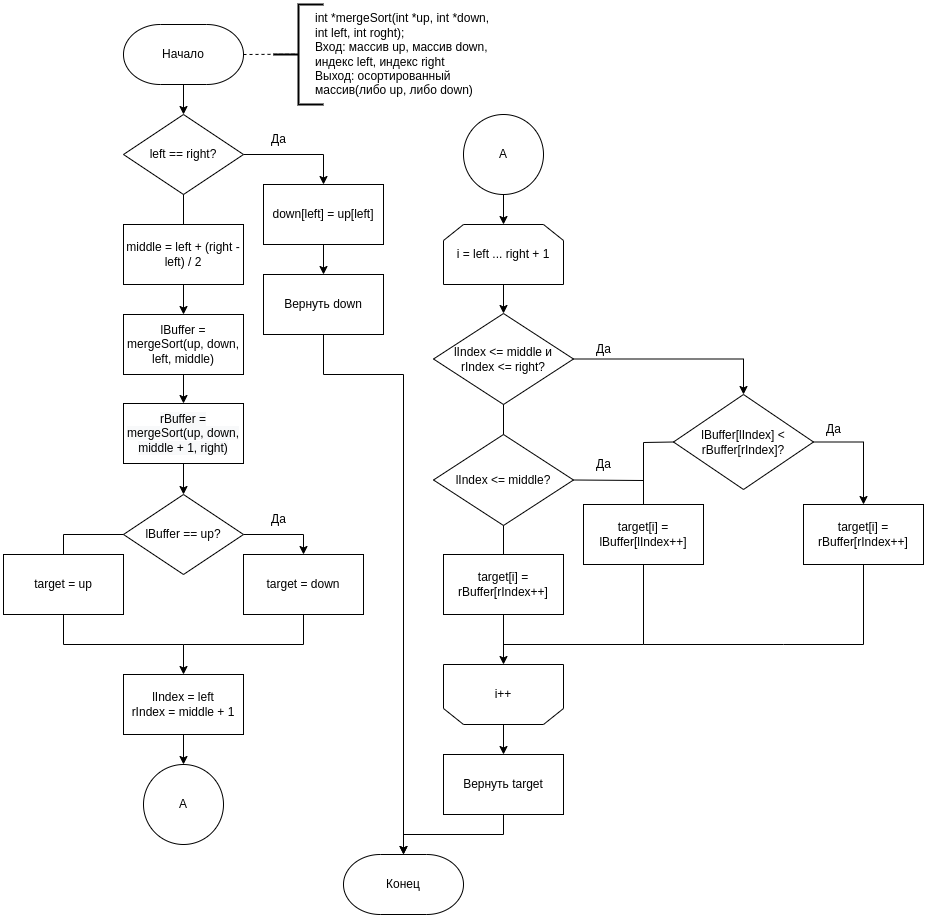
\includegraphics[width=170mm]{images/merge}
	\caption{Схема алгоритма сортировки слиянием.}
	\label{img:merge}
\end{figure}
\newpage
На рисунке \ref{img:counting} приведена схема алгоритма сортировки подсчетом.
\begin{figure}[h]
	\centering
	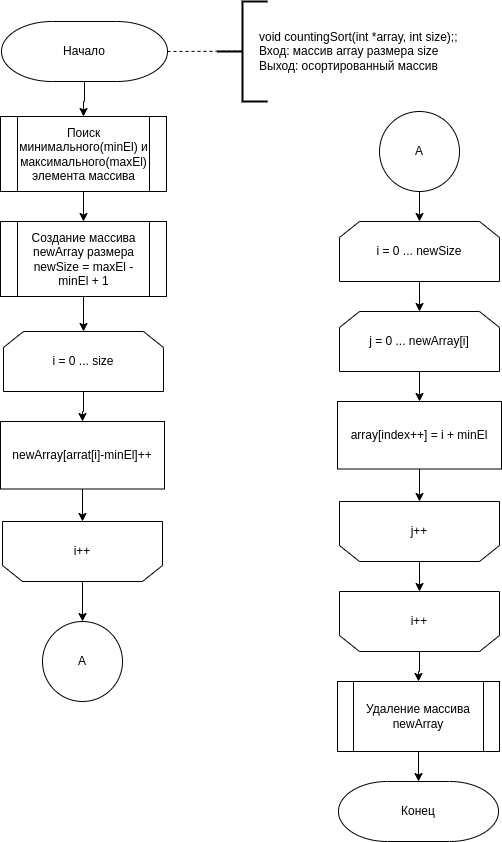
\includegraphics[width=110mm]{images/counting}
	\caption{Схема алгоритма сортировки подсчетом.}
	\label{img:counting}
\end{figure}

\newpage
На рисунке \ref{img:bitonic} приведена схема алгоритма битонной сортировки.
\begin{figure}[h]
	\centering
	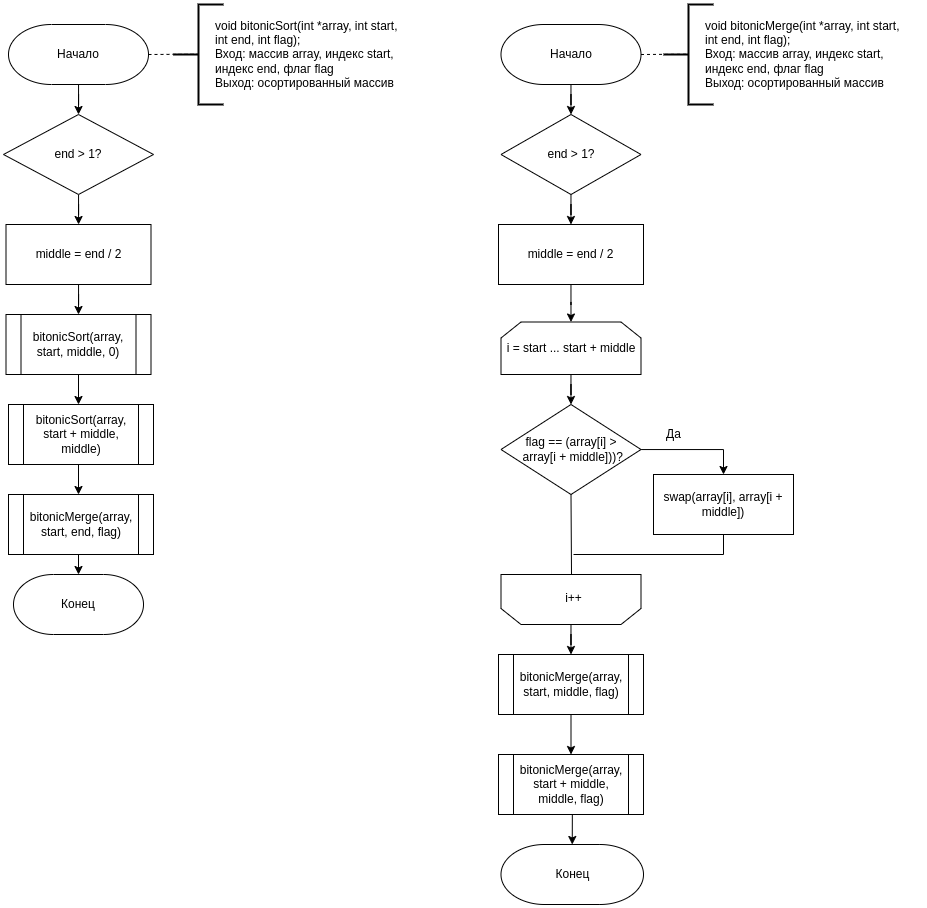
\includegraphics[width=175mm]{images/bitonic}
	\caption{Схема алгоритма битонной сортировки.}
	\label{img:bitonic}
\end{figure}

\section{Модель вычислений}